% ----------------------------------------------------------
% Seção Lógica - Principal
% ----------------------------------------------------------
\section{Lógica}
Segundo o dicionário online de Português Dicio\cite{dicio_logica}, a palavra lógica se refere a:
\begin{enumerate}
   \item Modo de raciocinar coerente que \underline{expressa uma relação de causa e consequência};
   \item Maneira coerente através da qual os \underline{fatos ou situações se encadeiam}. 
 \end{enumerate}
\bigbreak
A palavra lógica expressa uma relação de causa e consequência ou fatos encadeados. Pode-se distinguir como essência dessas duas definições o movimento, a mudança, a transição. A palavra lógica, em sua essência, se encaixa perfeitamente na definição do NADA − NÃO SER.  A lógica NÃO SER é consonante com o NADA, pois sua outra face É ilógica e imutável. Nessa dualidade, tem-se a existência fundamentada pela lógica que "nega a si", enquanto, por outro lado É ilógica, imutável e inexistente. A expressão "negação de si" refere-se à negação do SER - NÃO SER. 
\bigbreak
A lógica está centrada na mudança e a mudança está centrada naquilo que NÃO É, uma vez que aquilo que É não pode deixar de SER. A mudança demanda que, em algum momento, algo DEIXE DE SER o que fora a se transformar. Em \citeonline{brasilescola_parmenides}, Parmênides  o filósofo da unidade e da identidade do SER, diz que a contínua mudança é a principal característica do não ser. Para Parmênides o SER é uno, eterno, não gerado e imutável.

A lógica SER ilógica não a impede de NÃO SER.  Na dualidade SER e NÃO SER, o SER limita e define o NÃO SER \textit{ad infinitum}. É possível se aproximar da definição do SER enumerando e definindo infinitamente tudo o que ele NÃO É.

\bigbreak
\begin{figure}[hbtp]
\caption{Analogia da lógica primordial}
\label{fig:primordial_logic_representation}
\centering
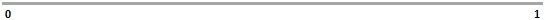
\includegraphics[scale=1]{sections/images/primordial_logic_representation.jpg}
\floatfoot{Reta utilizada para representar e validar o conceito da lógica primordial}%\footnotemark}
\end{figure}
%\footnotetext{Fonte: MathIsFun.com, 2019.}

\bigbreak
Na Figura \ref{fig:primordial_logic_representation} pode-se entender:
\begin{description}
   \item[{[1,1]}] esse ponto É ilógico, pois é a totalidade não fracionada da reta.
   \item[{[0,0]}] esse ponto É ilógico, pois é um ponto nulo incapaz de negar a si, dado que toda lógica ou sublógica (fração lógica) deve se manter negado a si, uma que essa é a premissa básica da lógica. A lógica NÃO É em sua essência, primordialmente.
   \item[$\textbf{{[0,1[ x ]0,1]}}$]a lógica é possível apenas na representação das frações ou intervalos dos pontos \textbf{0} e \textbf{1}. Uma fração da reta nega ser a reta, pois é apenas uma parte dela. Os subintervalos são hábeis a negar a si infinitamente, garantindo a premissa primordial da lógica e suas sublógicas, negar a si. 
\end{description}

\bigbreak
\begin{figure}[hbtp]
\caption{Primeiro momento lógico}
\label{fig:first_logical_moment}
\centering

\includegraphics[scale=1]{sections/images/first_logical_moment.jpg}
\floatfoot{Representação do primeiro momento lógico com a reta fracionada em dois intervalos. O segmento em azul representa a negação da lógica em SER o todo nesse primeiro momento }%\footnotemark}
\end{figure}
%\footnotetext{Fonte: MathIsFun.com, 2019.}

A união do traço à reta é a representação de um intervalo lógico, pois é da negação da lógica em SER que surgi esses intervalos. As duas frações geradas pela negação lógica negam SER a reta, pois são apenas intervalos delas e são capazes de negar a si infinitamente, garantindo a premissa primordial da lógica NÃO SER. 

% ----------------------------------------------------------
% Subseção Aspectos da Lógica
% ----------------------------------------------------------
\subsection{Aspectos da Lógica}
\lipsum[2]

\subsubsection{Expansão binomial}
\lipsum[2]

\subsubsection{Teorema central do limite}
\lipsum[2]


% ----------------------------------------------------------
% Subseção Aspectos da Consciência
% ----------------------------------------------------------
\subsection{Aspectos da Consciência}
\lipsum[2]

\subsubsection{Infinito}
\lipsum[2] 

\subsubsection{Tempo}
\lipsum[2]

\subsubsection{Espaço}
\lipsum[2]

\subsubsection{Gravidade}
\lipsum[2]

\subsubsection{Matéria e energia escuras}
\lipsum[2]

\subsubsection{Buraco negro}
\lipsum[2]


% ----------------------------------------------------------
% Subseção Especulação
% ----------------------------------------------------------
\subsection{Especulação}
\lipsum[2]